
\section{临界点的存在性}
\label{sec:critical-point-existence}

一个特殊的\trMinimax{}论证将保证上一节中所引入的\trFunctional{} $\Phi$ 的一个%
特殊\trCriticalPoint{}的存在性：
\[
\begin{aligned}
\Phi(x)\ &=\ a(x)-b(x)\\
&=\ \tfrac{1}{2}\|x^{+}\|^{2}-\tfrac{1}{2}\|x^{-}\|^{2}-\int_{0}^{1}%
H\bigl(x(t)\bigr)\,dt,
\end{aligned}
\]
其中 $x=x^{-}+x^{0}+x^{+}\in E=E^{-}\oplus E^{0}\oplus E^{+}$。回顾一下：%
$H\geq0$，并且 $H$ 在 $z=0\in\R^{2n}$ 的一个\trNeighborhood{}内恒为零。此外，%
对充分大的 $|z|$ 有 $H(z)=(\pi+\varepsilon)\,q(z)$。显然，函数 $H$ 的每个%
\trCriticalPoint{} $z\in\R^{2n}$——也就是 $\{z\mid\nabla H(z)=0\}$ 中的一点——%
都是 $\Phi$ 的满足 $\Phi(z)\leq0$ 的\trCriticalPoint。我们要寻找的，是 $\Phi$ 的%
那些并非常值\trLoop{}的\trCriticalPoint。

\begin{proposition}\label{prop:special-critical-point}
存在 $x^{*}\in E$ 满足 $\nabla\Phi(x^{*})=0$ 与 $\Phi(x^{*})>0$。
\end{proposition}

为了证明这个\trhProposition，我们先挑出 $E$ 的两个特定的子集 $\Sigma$ 与%
$\Gamma$。\trBounded{}集 $\Sigma=\Sigma_{\tau}\subset E$ 定义为
\[
\Sigma_{\tau}\ =\ \Bigl\{\,x\ \Bigm|\ x=x^{-}+x^{0}+se^{+}\ ,\ %
\|x^{-}+x^{0}\|\leq\tau\quad\text{以及}\quad 0\leq s\leq\tau\Bigr\}
\]
其中 $\tau>0$。这里 $e^{+}\in E^{+}$ 是元素
\[
e^{+}(t)=e^{2\pi Jt}\,e_{1}\qquad\text{以及}\qquad e_{1}=(1,0,\dots,0)\in\R^{2n}.
\]
显然 $\|e^{+}\|^{2}=2\pi$，而 $\|e^{+}\|_{L^{2}}=1$。我们以 $\partial\Sigma$ 表示%
$\Sigma$ 在 $E^{-}+E^{0}+\R e^{+}$ 中的\trBoundary。

\begin{lemma}\label{lem:boundary-sigma-negative}
存在 $\tau^{*}>0$，使得对 $\tau\geq\tau^{*}$ 有
\[
\Phi\big|_{\partial\Sigma}\ \leq\ 0.
\]
\end{lemma}

\begin{proof}
我们使用 $\Phi$ 的\trAsymptotic{}行为。由 $a\big|_{E^{-}\oplus E^{0}}\leq0$ 与%
$b\geq0$ 我们推得
\[
\Phi\big|_{E^{-}\oplus E^{0}}\ \leq\ 0.
\]
尚须考虑的，是\trBoundary{} $\partial\Sigma$ 中由 $\|x^{-}+x^{0}\|=\tau$ 或%
$s=\tau$ 所定义的那几部分。由 $H$ 的构造，存在常数 $\gamma>0$，使得
\[
H(z)\ \geq\ (\pi+\varepsilon)\,q(z)-\gamma\qquad\text{对一切}\quad z\in\R^{2n}.
\]
于是，
\[
\Phi(x)\ \leq\ a(x)-(\pi+\varepsilon)\int_{0}^{1}q(x)\,dt+\gamma\ ,\qquad%
\text{对一切}\quad x\in E.
\]
回顾\trQuadraticForm{} $q$ 的定义\footnote{原书两处积分漏排「$dt$」（$\int_{0}^{1}q(x)$ 与 $\int_{0}^{1}q(se^{+})$），此处径补。——译者注}，对\trOrthogonal{}分解%
$x=x^{-}+x^{0}+se^{+}\in E^{-}\oplus E^{0}+E^{+}$ 可以验证
\[
\int_{0}^{1}q\bigl(x^{-}+x^{0}+se^{+}\bigr)\,dt\ =\ \int_{0}^{1}%
q\bigl(x^{-}\bigr)\,dt+\int_{0}^{1}q\bigl(x^{0}\bigr)\,dt+\int_{0}^{1}%
q\bigl(se^{+}\bigr)\,dt\ .
\]
回顾 $\|e^{+}\|^{2}=2\pi$，我们便可以对 $x=x^{-}+x^{0}+se^{+}$ 作如下%
\trEstimate{}：
\begin{align*}
\Phi(x)\ &\leq\ \tfrac{1}{2}\,s^{2}\|e^{+}\|^{2}-\tfrac{1}{2}\|x^{-}\|^{2}-%
(\pi+\varepsilon)\,q\bigl(x^{0}\bigr)-(\pi+\varepsilon)\int_{0}^{1}%
q\bigl(se^{+}\bigr)\,dt+\gamma\\
&=\ -\tfrac{1}{2}\|x^{-}\|^{2}-\varepsilon s^{2}\,\|e^{+}\|^{2}_{L^{2}}-%
(\pi+\varepsilon)\,q\bigl(x^{0}\bigr)+\gamma.
\end{align*}
这样我们便找到一个常数 $c>0$，使得
\[
\Phi\bigl(x^{-}+x^{0}+se^{+}\bigr)\ \leq\ \gamma-c\,\|x^{-}+x^{0}\|^{2}-%
c\,\|se^{+}\|^{2}.
\]
当 $\tau$ 充分大时，只要 $\|x^{-}+x^{0}\|=\tau$ 或 $s=\tau$，右端便%
$\leq0$。这就完成了该引理的证明。
\end{proof}

子集 $\Gamma=\Gamma_{\alpha}\subset E^{+}$ 定义为
\[
\Gamma\ =\ \Bigl\{\,x\in E^{+}\ \Bigm|\ \|x\|\ =\ \alpha\Bigr\}.
\]

\begin{lemma}\label{lem:gamma-positive}
存在 $\alpha>0$ 与 $\beta>0$，使得
\[
\Phi\big|_{\Gamma}\ \geq\ \beta>0.
\]
\end{lemma}

\begin{proof}
我们使用 $\Phi$ 在 $x=0\in E$ 近旁的局部行为。回顾一下：$H$ 在 $\R^{2n}$ 中%
原点的近旁恒为零。我们将证明
\[
b(x)\,\frac{1}{\|x\|^{2}}\ \longrightarrow\ 0\qquad\text{当}\quad\|x\|\to0.
\]
于是，对 $x\in E^{+}$ 便得到
\[
\Phi(x)\,\frac{1}{\|x\|^{2}}\ =\ \frac{1}{2}-\frac{1}{\|x\|^{2}}\,b(x)%
\ \longrightarrow\ \frac{1}{2}\,.
\]
从而，只要 $\|x\|$ 充分小，便有 $\Phi(x)\geq\frac{1}{4}\|x\|^{2}$，这就蕴含了%
所要的结果。用反证法：我们找到一列 $x_{j}\in E$ 与一个常数 $d>0$，满足
\[
x_{j}\to0\qquad\text{以及}\qquad\frac{1}{\|x_{j}\|^{2}}\,b\bigl(x_{j}\bigr)%
\ \geq\ d>0.
\]
令 $y_{j}=x_{j}/\|x_{j}\|$，于是 $\|y_{j}\|=1$。我们断言：存在一个子序列%
$y_{j}$ 以及函数 $y$ 与 $w\in L^{2}$，满足
\begin{align*}
y_{j}\ &\longrightarrow\ y\qquad\text{在}\ L^{2}\ \text{中}\\
y_{j}(t)\ &\longrightarrow\ y(t)\\
\bigl|y_{j}(t)\bigr|\ &\leq\ w(t)\\
x_{j}(t)\ &\longrightarrow\ 0
\end{align*}
对\trAlmostEvery{}的 $t$ 成立。

的确，由\cref{prop:inclusion-map-compact}，$E$ 紧\trEmbedding{}于 $L^{2}$。%
于是我们能找到一个子序列 $y_{j}$，它在 $L^{2}$ 中是\trCauchy{}序列，而该论断%
便可由下面这个众所周知的论证得出。选出一个快速的\trCauchy{}子序列，我们不妨设
\[
\|y_{k+1}-y_{k}\|_{L^{2}}\ \leq\ \frac{1}{2^{k}}\ ,\qquad k\geq1.
\]
进而，由
\[
f_{n}(t):=\sum_{k=1}^{n}\bigl|y_{k+1}(t)-y_{k}(t)\bigr|,
\]
所定义的序列 $f_{n}\in L^{2}$ 单调递增，并且满足 $\|f_{n}\|_{L^{2}}\leq1$。%
于是由单调收敛定理，$f_{n}(t)$ 几乎处处\trConverge{}于 $f(t)$，且 $f\in L^{2}$。%
由于对 $m>n$ 有
\begin{align*}
\bigl|y_{m}(t)-y_{n}(t)\bigr|\ &\leq\ \bigl|y_{m}(t)-y_{m-1}(t)\bigr|+\dotsb+%
\bigl|y_{n+1}(t)-y_{n}(t)\bigr|\\
&\leq\ f(t)-f_{n-1}(t),
\end{align*}
我们便得出结论：对\trAlmostEverywhere{}的 $t$，序列 $y_{n}(t)$ 是 $\R^{2n}$ 中的%
\trCauchy{}序列\footnote{原书印作「$\R$ 中的 Cauchy 序列」，诸 $y_{n}(t)\in\R^{2n}$，此处径改。——译者注}，从而对\trAlmostEverywhere{}的 $t$ 定义了%
$y(t):=\lim y_{n}(t)$。鉴于 $|y(t)-y_{n}(t)|\leq f(t)$，我们借助\trLebesgue{}%
收敛定理进而得到：在 $L^{2}$ 中 $y_{n}\to y$；又由于对\trAlmostEverywhere{}的%
$t$ 有 $|y_{n}(t)|\leq f(t)+|y(t)|=:w(t)$，且 $w\in L^{2}$，该论断便得证。%
按定义，
\[
b\bigl(x_{j}\bigr)\,\frac{1}{\|x_{j}\|^{2}}\ =\ \int_{0}^{1}H\bigl(x_{j}\bigr)\,%
\frac{1}{\|x_{j}\|^{2}}\,dt.
\]
由对一切 $z\in\R^{2n}$ 成立的 $H(z)\leq M|z|^{2}$，我们推得
\[
H\Bigl(x_{j}(t)\Bigr)\frac{1}{\|x_{j}\|^{2}}\ \leq\ M\,w(t)^{2}
\]
对\trAlmostEvery{}的 $t$ 成立，于是 $L^{1}$ 函数 $w(t)^{2}$ 便是一个优函数。%
利用 $H$ 连同其直到二阶为止的各阶\trDerivative{}都在 $z=0$ 处为零，借助%
\trTaylor{}公式我们得到
\[
H\Bigl(x_{j}(t)\Bigr)\frac{1}{\|x_{j}\|^{2}}\ =\ O\Bigl(\bigl|x_{j}(t)\bigr|\Bigr)\,%
\bigl|y_{j}(t)\bigr|^{2}\ \longrightarrow\ 0
\]
对\trAlmostEvery{}的 $t$ 成立。于是，借助\trLebesgue{}定理，
\[
\int_{0}^{1}H\Bigl(x_{j}(t)\Bigr)\frac{1}{\|x_{j}\|^{2}}\,dt\ \longrightarrow\ 0\ ,%
\qquad j\to\infty.
\]
这与假设 $d>0$ 矛盾，于是\cref{lem:gamma-positive}得证。
\end{proof}

当然，证明中那个颇为笨拙的论证，若利用下面这条众所周知、却并非初等的%
\trSobolev{}\trEstimate，本来是可以避免的。空间 $\Hh{1}{2}(S^{1})$ 对每个%
$p\geq1$ 都连续\trEmbedding{}于 $L^{p}(S^{1})$。于是存在常数 $M=M_{p}$，使得
\[
\|u\|_{L^{p}}\ \leq\ M\|u\|_{1/2}\ ,\qquad u\in\Hh{1}{2}(S^{1})\ .
\]
其证明可在附录中找到。姑且承认这个\trEstimate{}并注意到对一切 $z\in\R^{2n}$%
有 $|H(z)|\leq c\,|z|^{3}$，我们便找到一个常数 $K>0$，使得
\[
\int_{0}^{1}\bigl|H\bigl(x(t)\bigr)\bigr|\,dt\ \leq\ c\,\|x\|_{L^{3}}^{3}\ \leq\ %
K\,\|x\|_{1/2}^{3}\ ,
\]
对一切 $x\in\Hh{1}{2}$ 成立。现在，若 $x\in E^{+}$\footnote{原书印作「$E_{+}$」（下标），此处径改为上标「$E^{+}$」。——译者注}，则%
$\Phi(x)\geq\frac{1}{2}\|x\|^{2}-K\|x\|^{3}$，引理便是显然的了。下面的这幅图%
（图 3.7）更为几何化地描绘了我们的处境。

\noindent\begin{minipage}{\linewidth}
\centering
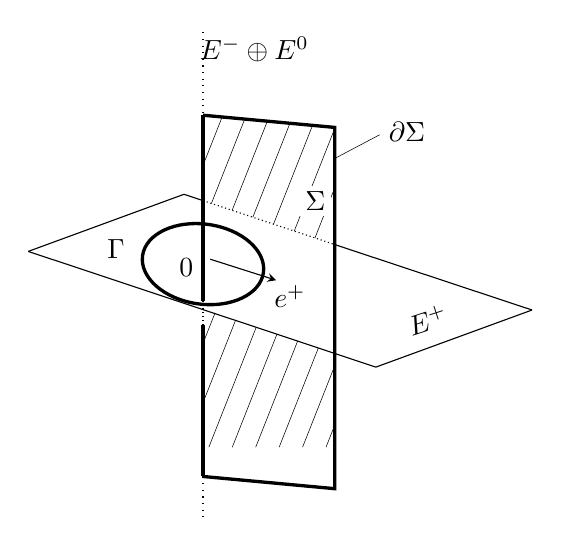
\begin{tikzpicture}[>=stealth,scale=0.62]
  \draw[dotted] (0,8.0) -- (0,6.3);%
  \draw[densely dotted] (0,2.5) -- (0,2.0);%
  \draw[dotted] (0,-1.1) -- (0,-2.0);%
  \begin{scope}
    \clip (0,6.3) -- (2.7,6.05) -- (2.7,3.65) -- (0,4.55) -- cycle;
    \foreach \i in {0,...,15}
      \draw[very thin] (-4.2+0.48*\i,-0.5) -- (-1.0+0.48*\i,7.6);
  \end{scope}
  \begin{scope}
    \clip (0,2.33) -- (2.7,1.42) -- (2.7,-1.35) -- (0,-1.1) -- cycle;
    \foreach \i in {0,...,15}
      \draw[very thin] (-4.2+0.48*\i,-0.5) -- (-1.0+0.48*\i,7.6);
  \end{scope}
  \draw[very thick] (0,6.3) -- (2.7,6.05) -- (2.7,-1.35) -- (0,-1.1);%
  \draw[very thick] (0,6.3) -- (0,2.5);%
  \draw[very thick] (0,2.0) -- (0,-1.1);%
  \draw (-3.58,3.51) -- (-0.39,4.68);%
  \draw (-0.39,4.68) -- (0,4.55);%
  \draw[densely dotted] (0,4.55) -- (2.7,3.65);%
  \draw (2.7,3.65) -- (6.74,2.31);%
  \draw (-3.58,3.51) -- (3.54,1.14);%
  \draw (3.54,1.14) -- (6.74,2.31);%
  \begin{scope}[rotate around={-8:(0,3.25)}]
    \draw[very thick] (0,3.25) ellipse [x radius=1.25, y radius=0.82];
  \end{scope}
  \draw[->] (0.15,3.35) -- (1.5,2.92);
  \node at (-0.34,3.18) {$0$};
  \node at (1.78,2.58) {$e^{+}$};
  \node at (-1.78,3.55) {$\Gamma$};
  \node at (1.05,7.65) {$E^{-}\oplus E^{0}$};
  \node[fill=white,inner sep=2pt] at (2.3,4.55) {$\Sigma$};
  \draw[very thin] (2.71,5.42) -- (3.62,5.9);%
  \node at (4.18,5.95) {$\partial\Sigma$};
  \node[rotate=18] at (4.6,2.1) {$E^{+}$};
\end{tikzpicture}

图 3.7
\end{minipage}

\trEstimate{} $\Phi\big|_{\partial\Sigma}\leq0$ 反映了我们对原来的%
\trHamiltonianFunction{} $H\in\mathcal{H}(Z(1),\omega_{0})$ 所作的假设%
$H\geq0$ 与 $m(H)>\pi+\varepsilon$，而 $\Phi\big|_{\Gamma}\geq\beta>0$ 则是%
下述假设的推论：$H$ 在某个开集上恒为零，而这个开集我们可以选成 $\R^{2n}$ 中%
原点的一个\trNeighborhood。

接下来我们研究：如果我们借助属于 $E$ 上\trGradient{}方程%
$\dot{x}=-\nabla\Phi(x)$ 的\trFlow{} $\varphi^{t}(x)$ 来平移集合 $\Sigma$，%
将会发生什么。由于 $\Phi\bigl(\varphi^{t}(x)\bigr)$ 关于 $t$ 递减，我们立即由%
\cref{lem:boundary-sigma-negative}得出
\begin{equation}\label{eq:phi-boundary-translate}
\Phi\big|_{\varphi^{t}(\partial\Sigma)}\ \leq\ 0\qquad\text{对一切}\quad t\geq0.
\end{equation}
而另一方面，由\cref{lem:gamma-positive}有 $\Phi\big|_{\Gamma}>0$，从而对一切%
$t\geq0$ 有 $\varphi^{t}(\partial\Sigma)\cap\Gamma=\varnothing$；随着 $t$ 增大，%
「框架」$\varphi^{t}(\partial\Sigma)$ 不能穿越「\trCircle」$\Gamma$。因此，%
直觉上清楚的是：由该框架所张成的「\trSurface」$\varphi^{t}(\Sigma)$ 必定对%
每个 $t\geq0$ 都与 $\Gamma$ 相交。然而这需要一个证明，它将基于一个%
\trTopology{}论证。

\begin{lemma}\label{lem:flow-sigma-intersects-gamma}
对一切 $t\geq0$ 有 $\varphi^{t}(\Sigma)\cap\Gamma\neq\varnothing$。
\end{lemma}

我们把它的证明往后放一放，先来完成\cref{prop:special-critical-point}的证明。%
事实上，此刻我们已经万事俱备。我们可以应用下述\trMinimax{}论证：取由诸子集%
$\varphi^{t}(\Sigma)$（对每个 $t\geq0$）所组成的族 $\mathcal{F}$，并定义
\[
c(\Phi,\mathcal{F})\ =\ \inf_{t\geq0}\ \sup_{x\in\varphi^{t}(\Sigma)}\ \Phi(x).
\]
我们断言 $c(\Phi,\mathcal{F})$ 是有限的。的确，由于%
$\varphi^{t}(\Sigma)\cap\Gamma\neq\varnothing$ 且 $\Phi\big|_{\Gamma}\geq\beta$，%
我们得出结论
\[
\beta\ \leq\ \inf_{x\in\Gamma}\Phi(x)\ \leq\ \sup_{x\in\varphi^{t}(\Sigma)}%
\Phi(x)\ <\ \infty.
\]
对于第二个\trEstimate，我们用到了：$\Phi$ 把\trBounded{}集映为\trBounded{}集%
（鉴于\cref{lem:gradient-b-compact}）。于是，
\[
-\infty\ <\ \beta\ \leq\ c(\Phi,\mathcal{F})\ <\ \infty.
\]
我们已经知道，\trFunctional{} $\Phi$ 满足\trPalaisSmale{}条件%
（\cref{lem:palais-smale-condition}），而且\trGradient{}方程生成一个唯一的%
整体\trFlow{}（\cref{lem:gradient-flow-representation}）。此外，由不依赖时间的%
方程所确定的\trFlow{}的性质，族 $\mathcal{F}$ 是正\trInvariant{}的。于是，%
\trMinimax{}引理便保证 $c(\Phi,\mathcal{F})$ 是一个\trCriticalValue。我们推得：%
存在一点 $x^{*}\in E$ 满足 $\nabla\Phi(x^{*})=0$ 与
\[
\Phi\bigl(x^{*}\bigr)\ =\ c(\Phi,\mathcal{F})\ \geq\ \beta>0,
\]
于是\cref{prop:special-critical-point}得证。尚待证明的是%
\cref{lem:flow-sigma-intersects-gamma}。

\begin{proof}[\cref*{lem:flow-sigma-intersects-gamma}的证明]
我们将使用\trLeray-\trSchauder\trDegree。这个度把\trBrouwer\trMapping\trDegree{}%
延拓到无穷维空间，其适用对象限于由形如 $\id+\text{紧}$ 的连续映射所组成的%
受限的类。把该\trFlow{}简记为 $\varphi^{t}(x)\equiv x\cdot t$，我们想验证：%
对一切 $t\geq0$ 有 $(\Sigma\cdot t)\cap\Gamma\neq\varnothing$。我们可以把它%
改写成如下要求：
\begin{equation}\label{eq:fixed-point-system}
\begin{aligned}
\bigl(P^{-}+P^{0}\bigr)(x\cdot t)\ &=\ 0\\
\|x\cdot t\|\ &=\ \alpha\\
x\ &\in\ \Sigma\ .
\end{aligned}
\end{equation}
回顾一下：由\cref{lem:gradient-flow-representation}，该\trFlow{}具有表示%
$x\cdot t=e^{t}x^{-}+x^{0}+e^{-t}x^{+}+K(t,x)$，于是%
\eqref{eq:fixed-point-system} 变成
\begin{equation}\label{eq:fixed-point-system-2}
\begin{aligned}
0\ &=\ e^{t}x^{-}+x^{0}+\bigl(P^{-}+P^{0}\bigr)K(t,x)\\
0\ &=\ \alpha-\|x\cdot t\|\\
x\ &\in\ \Sigma\ .
\end{aligned}
\end{equation}
把 $E^{-}$ 部分乘以 $e^{-t}$，便得到等价的方程
\begin{equation}\label{eq:fixed-point-system-3}
\begin{aligned}
0\ &=\ x^{-}+x^{0}+\bigl(e^{-t}P^{-}+P^{0}\bigr)K(t,x)\\
0\ &=\ \alpha-\|x\cdot t\|\\
x\ &\in\ \Sigma\ .
\end{aligned}
\end{equation}
由于 $x\in\Sigma$ 可表示为 $x=x^{-}+x^{0}+se^{+}$（$0\leq s\leq\tau$），%
我们可以把 \eqref{eq:fixed-point-system-3} 改写如下：
\begin{equation}\label{eq:fixed-point-equation}
0\ =\ x+B(t,x)\qquad\text{以及}\qquad x\in\Sigma,
\end{equation}
其中\trOperator{} $B$ 定义为
\[
B(t,x)\ =\ \bigl(e^{-t}P^{-}+P^{0}\bigr)K(t,x)+P^{+}\Bigl\{\Bigl(\|x\cdot t\|-%
\alpha\Bigr)e^{+}-x\Bigr\}.
\]
简记 $F=E^{-}\oplus E^{0}+\R e^{+}$，则映射 $B:\R\times F\to F$ 连续，并把%
\trBounded{}集映入相对\trCompact{}的集合；这是在\cref{lem:gradient-flow-representation}中%
证明了的。因此我们可以应用\trLeray-\trSchauder{}指标理论。只要我们能证明%
$\deg\bigl(\Sigma,\id+B(t,\cdot),\,0\bigr)\neq0$，方程%
\eqref{eq:fixed-point-equation} 对给定的 $t\geq0$ 便拥有解 $x\in\Sigma$。%
为了计算这个度，我们首先注意到：鉴于对 $t\geq0$ 有%
$\varphi^{t}(\partial\Sigma)\cap\Gamma=\varnothing$，%
\eqref{eq:fixed-point-equation} 在 $\partial\Sigma$ 上没有解，也就是说，
\[
0\ \notin\ \bigl(\id+B(t,\cdot)\bigr)(\partial\Sigma)\ ,
\]
其中 $t\geq0$。于是，依据\trDegree{}的\trHomotopy\trInvariance，
\[
\deg\bigl(\Sigma,\id+B(t,\cdot),\,0\bigr)\ =\ %
\deg\bigl(\Sigma,\id+B(0,\cdot),\,0\bigr).
\]
由于 $K(0,x)=0$，我们得到 $B(0,x)=P^{+}\bigl\{(\|x\|-\alpha)e^{+}-x\bigr\}$。%
定义\trHomotopy
\[
L_{\mu}(x)\ =\ P^{+}\Bigl\{\bigl(\mu\|x\|-\alpha\bigr)\,e^{+}-\mu x\Bigr\}%
\qquad\text{对}\quad 0\leq\mu\leq1,
\]
我们断言：对 $x\in\partial\Sigma$ 有 $x+L_{\mu}(x)\neq0$。的确，若%
$x\in\Sigma$ 满足 $x+L_{\mu}(x)=0$，则 $x=se^{+}$，从而%
$s\bigl((1-\mu)+\mu\|e^{+}\|\bigr)=\alpha$。于是 $0<s\leq\alpha$，故当%
$\tau>\alpha$ 时 $x\notin\partial\Sigma$，如所断言。因此，再次依据\trHomotopy，
\begin{align*}
\deg\bigl(\Sigma,\id+B(t,\cdot),\,0\bigr)\ &=\\
\deg\bigl(\Sigma,\id+L_{0},\,0\bigr)\ &=\\
\deg\bigl(\Sigma,\id-\alpha e^{+},\,0\bigr)\ &=\\
\deg\bigl(\Sigma,\id,\,\alpha e^{+}\bigr)\ &=\ 1,
\end{align*}
只要 $\alpha e^{+}\in\Sigma$——这对 $\tau>\alpha$ 成立。这就完成了%
\cref{lem:flow-sigma-intersects-gamma}的证明，从而该\trhProposition{}的证明也%
告完成。
\end{proof}

在该\trhProposition{}中所找到的这个\trCriticalPoint{}是 $\R^{2n}$ 中%
\trHamiltonianEquation{} $\dot{z}=J\nabla H(z)$ 的一个\trPeriodic{}为 $1$ 的%
\trSmooth\trPeriodicSolution，正如我们从那个「\trRegularity」的%
\cref{lem:critical-point-regularity}所知道的。这个解便是我们在%
\cref{thm:z1-period-1}中所寻找的那个特定的非常值 $1$\trPeriodicSolution，%
因此该定理的证明至此完成。借助这个关于\trPeriodicSolution{}的存在性定理，%
我们同时也建立了特殊的\trCapacity{}函数 $c_{0}(M,\omega)$ 的存在性。从而，%
上一章中从某个\trCapacity{}函数 $c$ 的存在性所推得的那些\trRigidity{}结果，%
现在便完全获证。我们已经证明：辛几何中这些晚近发现的\trRigidity{}现象，%
可以追溯到施加于\trClassicalMechanics{}那个古老的\trAction{}原理的一个简单的%
\trMinimax{}论证。
